\documentclass{standalone}
\usepackage{pgfplots}
\pgfplotsset{compat=newest}

\pagestyle{empty}

\begin{document}
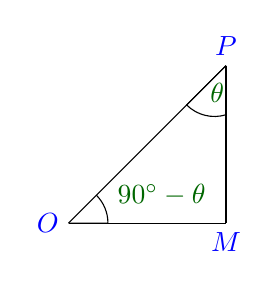
\begin{tikzpicture}
\draw (0, 0) -- (2, 0);
\draw (0, 0) -- (2, 2);
\draw (2, 0) -- (2, 2);
\draw [blue] (0, 0) node[anchor=east] {$O$};
\draw [blue] (2, 0) node[anchor=north] {$M$};
\draw [blue] (2, 2) node[anchor=south] {$P$};
\draw (0, 0) -- (0.5, 0) arc[start angle=0, end angle=45, radius=0.5];
\draw (2, 2) -- (1.5, 1.5) arc[start angle=225, end angle=287, radius=0.5];
\draw [black!60!green] (0.5, .1) node[anchor=south west] {$90^\circ - \theta$} ;
\draw [black!60!green] (2.1, 1.9) node[anchor=north east] {$\theta$};
\end{tikzpicture}
\end{document}
